% Chapter 7
\section*{Preface}

\pagebreak

\chapter{Impact of solvents and current collectors on rechargeable AIBs} % Main chapter title
\label{chap7} % For referencing the chapter elsewhere, use \ref{Chapter1} 

\section{Theory and background}
Battery electrodes are manufactured by casting a slurry onto a current collector. The slurry contains an active material, conductive carbon, a binder dispersed in a solvent, also known as a dispersing agent. A good solvent should provide high viscosity, high stability, high dispersity, avoid decomposition of electrolyte and improve the compatibility of cathode slurry and electrolyte\cite{ludwig_solvent-free_2016}. No agglomeration of the particulate materials should be allowed because that leads to a poorly flowing slurry. A poorly dispersed slurry leads to a non-uniform coating on the current collector , which would give an uneven weight distribution. This will deteriorate the battery performance and a slower transfer of energy to or from the cell. N-methyl pyrrolidone (NMP) has been a popular choice as an organic solvent used in slurries because of its many advantages. It is a polar solvent and its functional groups provide enhanced adhesion with binders, especially PVDF. It's vapor pressure or boiling point is not very low (Table \ref{t1}) , giving a good electrode quality and enhances scalability of cell fabrication. 
After the slurry has been mixed uniformly, it is cast onto Mo foil and dried. Solvent evaporation is necessary for cell fabrication. Ideally, an NMP recovery system must be in place during the drying process to recover evaporated NMP due to the high cost and potential pollution of NMP. While the recovery system makes the entire process more economical, it does require a large capital investment. Less expensive solvents could eliminate the large capital cost of the recovery system. Unconventional cathode manufacturing techniques have been used to coat current collectors with electrode material. \cite{liu_effective_2014-1,spreafico_pvdf_2014-1, liu_effects_2008-1, lee_effect_2010-1, wenzel_challenges_2015}.
\section{Experimental methods}
A slurry was prepared by mixing the active material (hBN) and carbon black in a vial. In a separate vial, PVDF and the solvent was mixed together to obtain a viscous solution. The two were then mixed together overnight. Once the slurry is prepared, it was coated on a current collector. After coating the foils with the slurry, the electrodes were dried at 80$^{\circ}$C for two hours and then vacuum dried at 120$^{\circ}$C for 12 hours. It is essential that the solvent evaporates and is completely removed from the coated electrode.  
\section{Results and discussions}
\subsection*{Solvents}
The electrode-electrolyte interface influences the battery performance. The solvent is crucial in determining the slurry quality and cathode's surface morphology. The standard solvent used was NMP, which provided a homogeneous mixture and a smooth surface after vacuum drying. Table \ref{t1} shows the list of solvents investigated for making hBN slurries. The ratio of active material, conductive carbon and the binder was kept constant (85:9:6). A good binder-solvent combination facilitates homogeneous dispersion of the slurry on a current collector. It was essential for the solvent to dissolve PVDF for proper performance of a battery. The binder needs to be dispersed uniformly on the metal foil for proper adhesion of the slurry \cite{lee_selection_2017, stein_non-aqueous_2016}. 
NMP is expensive , therefore scientists have always looked for alternatives. The NMP/PVDF couple was replaced by water/ elastomers (styrene-butadiene rubber, \cite{lee_novel_2007, li_effects_2005} in LIBs, however the anode was not compatible with water. Since we use aluminium as an anode, water cannot be used as a solvent because it would react with aluminium forming oxides and corrode it.
\begin{table}
\caption{List of solvents used for making cathode slurries.} \label{t1}
\begin{center}
 \begin{tabular}{|ccccc|} 
 \hline
 \textbf{Solvent} & \textbf{Polarity} & \textbf{Boiling point} & \textbf{Price}\\
 \textbf{} & \textbf{} & \textbf{($^{\circ}$C)} & \textbf{(\$/ L$^{-1}$)}\\
 \hline
 \hline
IPA & 0.55 & 82 & 83 \\
Toluene & 0.09 & 110 & 88 \\
Acetone & 0.35 & 56 & 93 \\
Methanol & 0.76 & 65 & 112 \\ 
Butanol & 0.59 & 117 & 143 \\
DMSO & 0.44 & 189 & 198 \\
DMF & 0.39 & 153 & 207 \\
DMA & 0.35 & 165 & 211 \\
Acetonitrile & 0.35 & 82 & 221 \\
NMP & 0.35 & 202 & 259 \\
 \hline
\end{tabular}
\end{center}
\end{table}
A few slurries we obtained using different solvents were visibly different. It was observed that dimethylsulfoxide (DMSO), dimethylformamide (DMF), dimethylacetamide (DMA) and NMP resulted in clear solutions after mixing with PVDF, while ethanol, isopropanol, toluene, acetone, methanol and butanol resulted in a cloudy solution. 
However, it turned out that boiling point of the solvents was a limiting factor. High volatility of the solvents resulted in quick drying of the slurries. Solvents with low boiling points such as acetone, ethanol, methanol isopropanol and acetonitrile did not allow a smooth coating of the slurries. High evaporation rates caused rapid drying of the coating, which resulted in formation of cracks before they could be vacuum dried.
The remaining slurries based on DMSO, DMF, DMA, NMP, butanol and toluene were casted and dried according to the process described above. Toluene and butanol resulted in a cracked film quality similar to the one with other high-volatile solvents. Consequently, the cathodes left for further electrochemical tests were the ones made from DMSO, DMF and DMA.
The cathodes were tested via galvanostatic charge/discharge cycles in Figure \ref{Figures/chap7fig:hBNsolvents}. Since we used hBN as the standard material, most of the solvents showed similar results. Figure \ref{Figures/chap7fig:hBNsolvents}b  shows that overall capacity of DMA based cathode was highest in its first cycle. However, it also recorded the highest capacity fading. A possible explanation could be deducted from the coulombic efficiencies shown in Figure \ref{Figures/chap7fig:hBNsolventsCE}b. With efficiencies higher than 100\% for almost every cycle, it is likely that a few additional reactions took place, which also resulted. However, DMSO based hBN cathodes showed consistent but high cell efficiencies >100\%. 
\begin{figure}[tbh!]
\centering
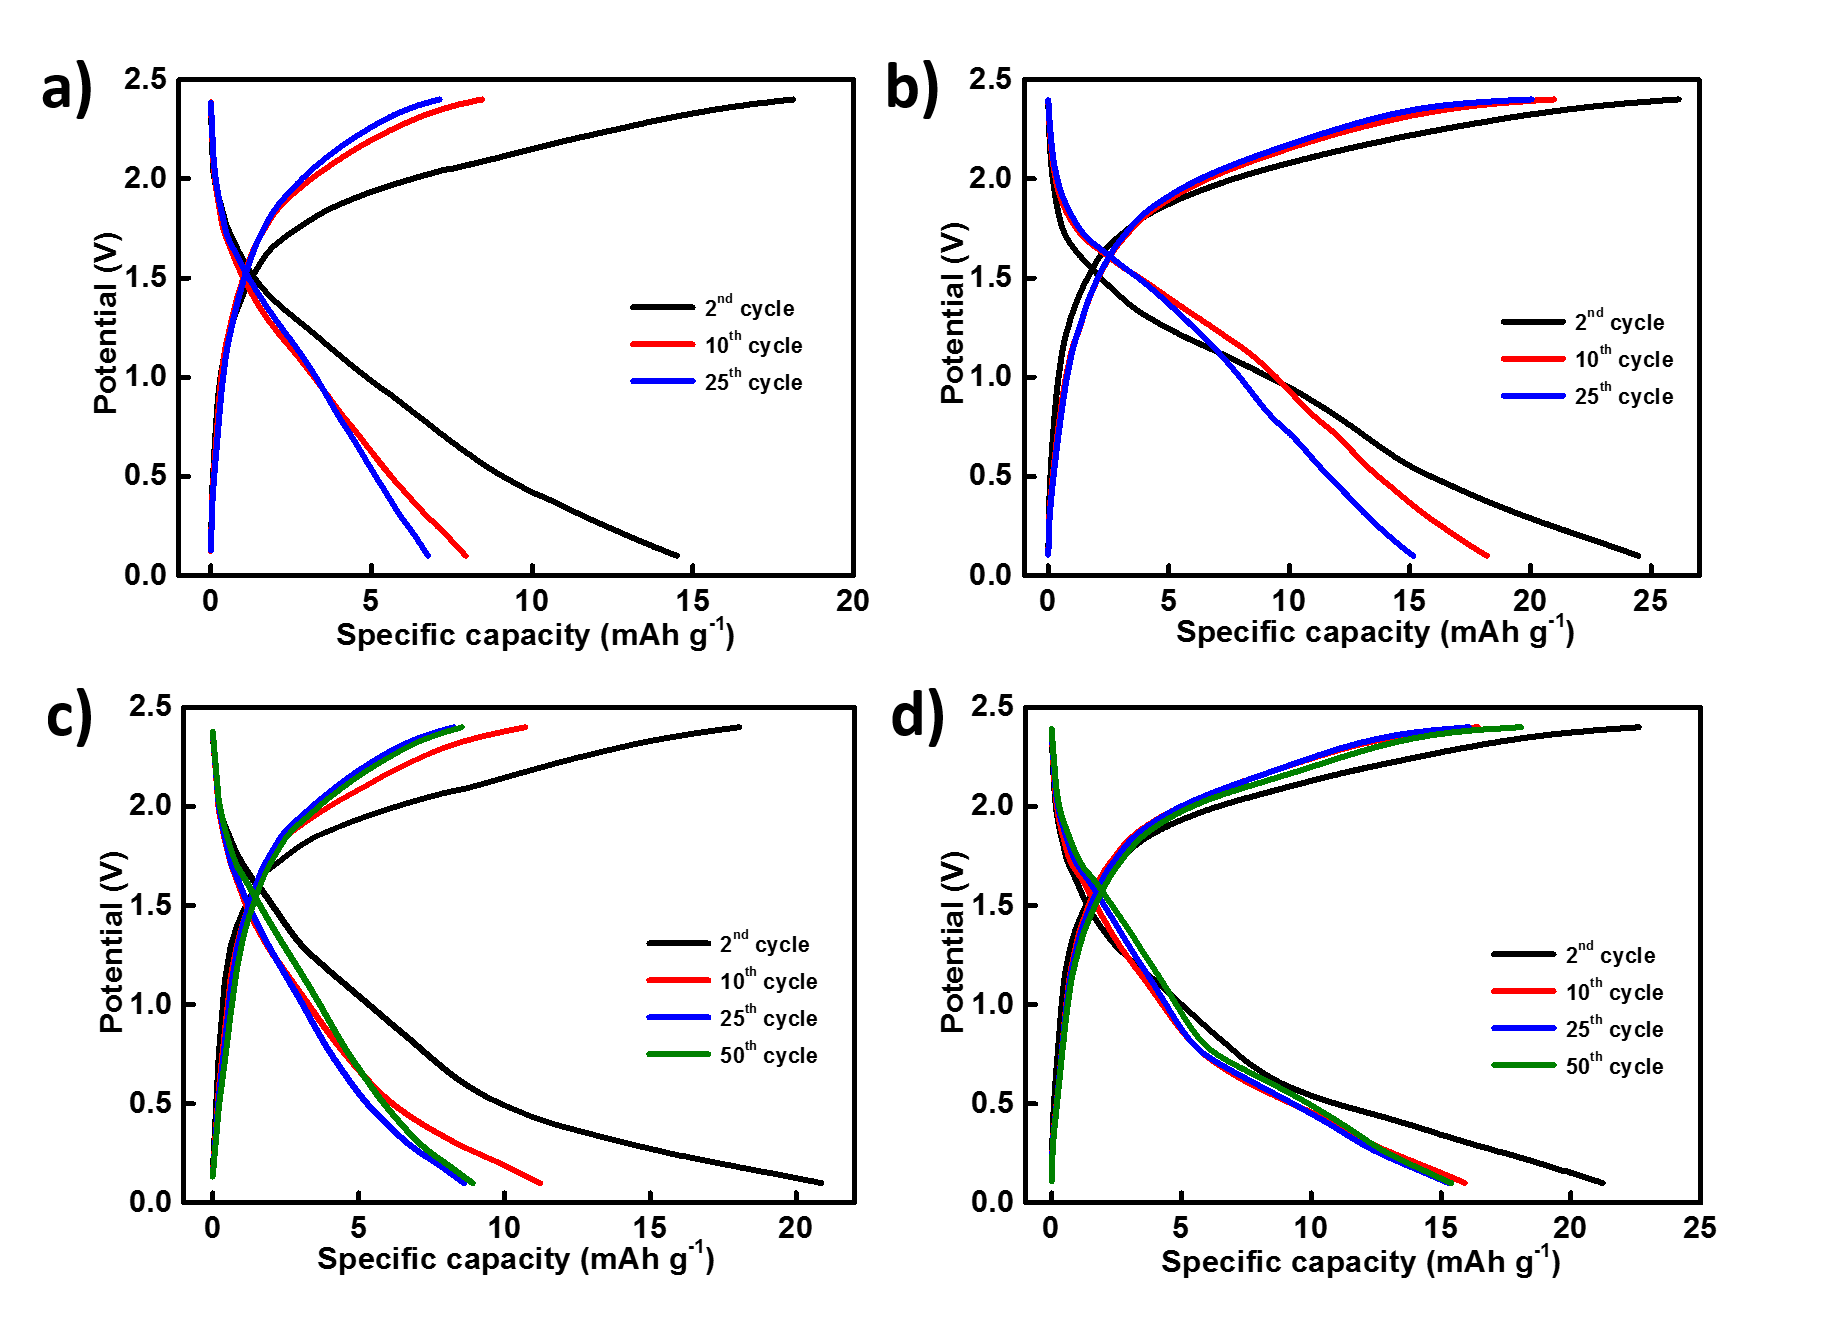
\includegraphics[width=\textwidth]{Figures/chap7fig/hBNsolvents}
\caption{Galvanostatic CDCs of Al/hBN cells using different solvents, a) DMSO, b) DMA, c) DMF and d) NMP.}
\label{Figures/chap7fig:hBNsolvents}
\end{figure}
\begin{figure}[tbh!]
\centering
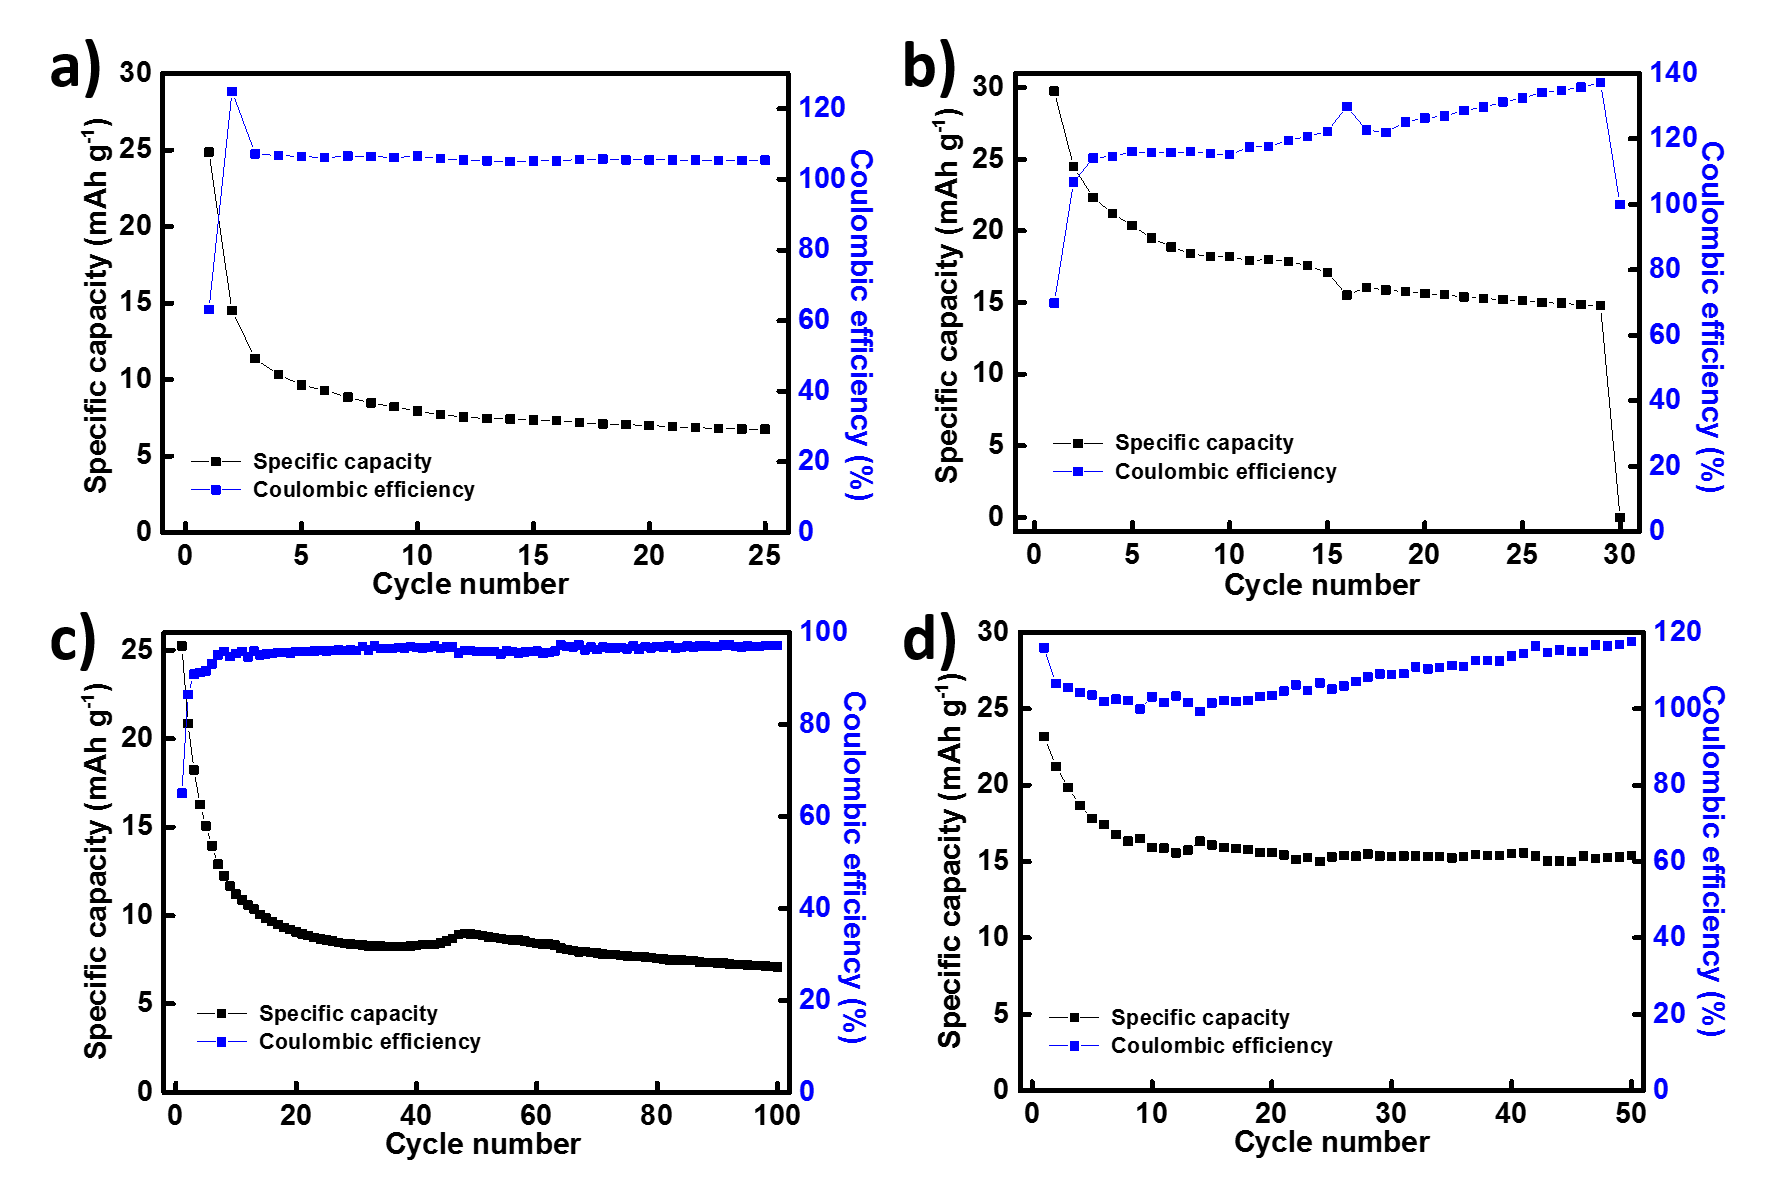
\includegraphics[width=\textwidth]{Figures/chap7fig/hBNsolventsCE}
\caption{Performance of Al/hBN cells using different solvents, a) DMSO, b) DMA, c) DMF and d) NMP.}
\label{Figures/chap7fig:hBNsolventsCE}
\end{figure}
Comparing DMF and NMP-based cathodes showed that with increasing cycle numbers capacity of DMF-based cathode decreased significantly faster compared to the NMP based cathode. Though, cell efficiency for DMF (98\%) was better than that for NMP-based cathode (>100\%).
\begin{figure}[tbh!]
\centering
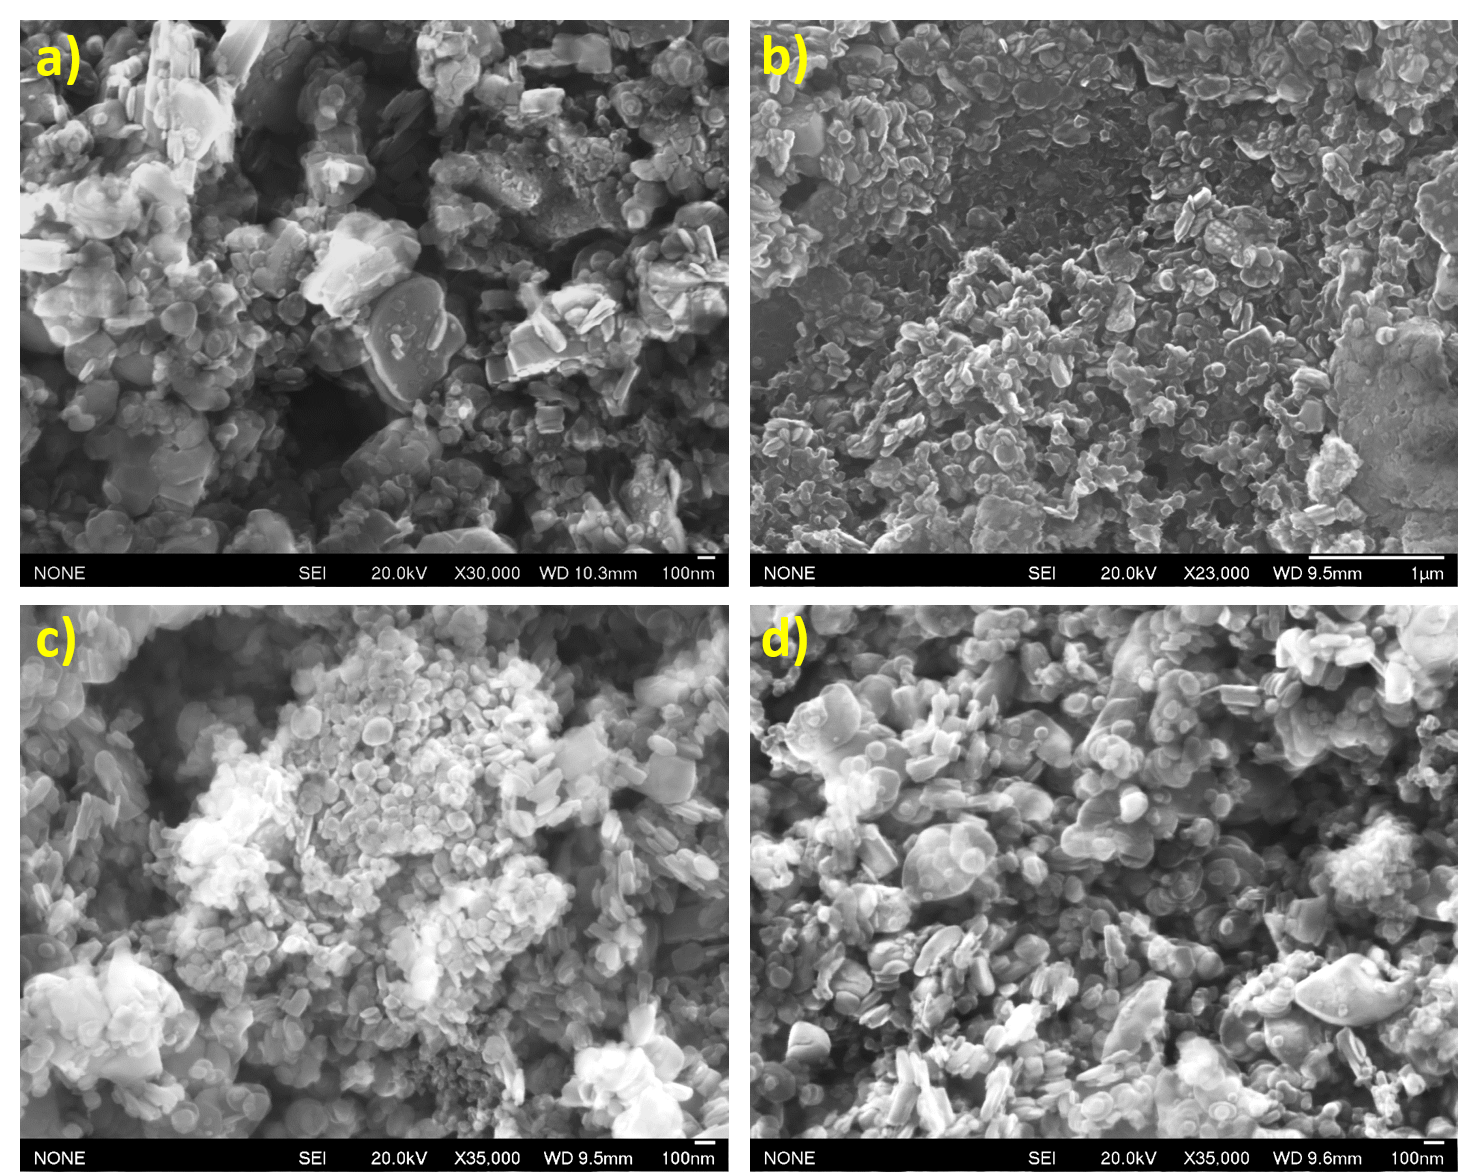
\includegraphics[width=\textwidth]{Figures/chap7fig/hBNsolventSEM}
\caption{SEM images of pristine hBN cathodes using a) DMSO, b) DMA, c) DMF and d) NMP solvents.}
\label{Figures/chap7fig:hBNsolventSEM}
\end{figure}
To study the impact of solvents on cathode morphology, we compared SEM images in Figure \ref{Figures/chap7fig:hBNsolventSEM}. Cathodes using DMSO and DMA (Figure \ref{Figures/chap7fig:hBNsolventSEM}a and b, showed agglomerated particles of hBN. Cathodes made of DMF and NMP did not agglomerate and retained the hexagonal shape of hBN. Overall, DMF showed a consistent discharge capacity after 50 cycles, a very high coulombic efficiency and retained the cathode structure. It can be used as an alternative to NMP , which would reduce the battery assembly cost. 
\subsection*{Current collectors}
\begin{table}
\caption{List of materials used as current collectors in increasing order of their marker price.} \label{t2}
\begin{center}
 \begin{tabular}{|cccc|} 
 \hline
 \textbf{Material} & \textbf{Thickness} & \textbf{Price} & \textbf{Conductivity} \\
 \textbf{Material} & \textbf{(mm)} & \textbf{(\$)} & {X 10$^{7}$}({$\Omega$}m)$^{-1}$ \\
  \hline
 \hline
Steel & 0.1 & 1.0 & 0.6 \\ 
Carbon paper & <0.1 & 1.2 & 6.5 \\
Aluminium & 0.1 & 3.04 & 3.6 \\
Brass & 1 & 5.07 & 1.4 \\
Copper & 0.1 & 9.91 & 5.9 \\ 
Nickel foam & 1 & 17.93 & 1.4 \\
Molybdenum & 0.1 & 39.61 & 1.9 \\
\hline
\end{tabular}
\end{center}
\end{table}
A current collector is a conductive solid connected to the electrode with external loading. The primary role of a current collector is to provide support to the electrodes (cathode and/or anode), collect the accumulated electrical energy from the electrode. A common current collector is a metal foil onto which a slurry is coated. A good connection between the active material and the metal foil is established only after a slow drying process which evaporates the solvent and binds it to the CC. Many metal foils have been used as metal/alloys foils in LIBs, such as nickel, copper, aluminium and steel. LIBs use two metal foils. Copper is used for the anode and aluminium is used for the cathode. This is because the two metal foils are stable at different potentials. Copper is electrochemically stable at a lower potential--
 V vs. Li\ce{Li+}, whereas aluminium is stable at a higher potential-1.34 V vs. Li\ce{Li+}. Aluminium cannot be used in our setup because it acts an anode and any contact between the active material and the anode would create a short circuit.  A CC should allow a stable flow of electrons, and should be ionically insulated. A good CC should be mechanically robust, and freestanding (usually with a macroscale size). Since a CC should be electrochemically inert, we could not use nickel foil because it oxidised at 1.1 V vs. Al/\ce{Al3+}. Steel, which is light in weight and cheap, underwent a vigorous reaction with our electrolyte and resulted in undesirable products, which resulted in rapid capacity decay and a very short cycle life. It seemed that \ce{AlCl3}/EmImCl corroded in presence of steel as can be seen in Figure \ref{Figures/chap7fig:steeleffect}. To avoid this, a CC should be within the electrochemical window if the electrolyte being used. Chemical potential of a CC ({$\mu${${_{cc}}$}} < 2.5 V) vs. Al/\ce{Al$^{3+}$}. Molybdenum foil ticked all the boxes and therefore was chosen as the CC in all our battery tests.  
 We compared the cell performances of all cells using different CCs, showed in Figure \ref{Figures/chap7fig:hBNCCCDC}. Firstly, carbon as a CC stands out from the other CCs. The cell recorded the highest discharge capacity at 82 mAh g$^{-1}$ (in green). When run for longer, the capacity was retained at 70 mAh g$^{-1}$ after25 cycles. The curve was exceptionally similar to the CDCs of an Al/graphite cell (inset Figure \ref{Figures/chap7fig:hBNCCCDC}b). This lead us to the conclusion that hBN became dormant in this cell and graphitic nature of the carbon paper took over and acted as the active material intercalating the \ce{AlCl4-} ions during charge. Steel, nickel, copper, brass and copper foils did not allow any charge or discharge to take place. Despite applying a continuous current, the charges seemed to accumulate and provided an unstable flow of electrons. Copper is a highly conductive metal; when aluminium electroplates, a few ions might get deposited on the CC creating a short circuit. Steel on the other hand contains chromium, which reacts with \ce{AlCl3}/EmImCl and some greenish stuff can be observed after we open the cell Figure \ref{Figures/chap7fig:steeleffect} \cite{reed_roles_2013}. This confirms that a side reaction took place, which consumed the electrolyte. Brass is less conductive than copper, as seen in Table \ref{table2}, and it contains other metals which have impeded the cell reaction and its capacity.   
%The battery performance results are shown in figure 6. It can be seen that the charging behaviour of brass, copper and aluminium have a similar tendency. Starting from different voltages, charging the system does not result in an actual increase in voltage, thus charge built-up as desired. As shown in figure 6 a), brass, copper and aluminium tend to reach a specific equilibrium voltage regardless of the energy provided to the system. Energy consumption without any charging indicates other processes being present consuming the provided energy. It is assumed that the energy consumed is used to disintegrate the substrate material. Ideally, the substrate is not in direct contact with the electrolyte. In reality however there will always be some sort of contact area present. The Al atoms in the aluminium and eventually the iron or chromium atoms present in the brass and copper are resulting in the disintegration of the substrates as such. As a reference how a single charging/discharging cycle should appear, figure 6 b)	shows a complete cycle for a BN RAB using a molybdenum substrate. Here the desired charge built-up can be observed until reaching the cut-off limit of 2.4V and the following discharging can be observed. A very unique charging behaviour could be observed for carbon coated aluminium as a substrate for the hBN slurry as shown in figure 6 c). A mixture of fast charging and abrupt rapid discharging can be observed. Knowing the tendency of the aluminium shown in figure 6 a) to completely discharge to the cutoff voltage of 0.1, it can be assumed that the rapid discharging behaviour results from the underlying aluminium. As discussed in section 2, carbon based RAB have been shown to work well and achieve high charging rates. Therefore it is assumed that the charging phases are either caused by the BN cathode material or by the underlying carbon coating. Even though the just discussed tested alternatives did not succeed in charging at all, Ni foam and Carbon paper did successfully charge and discharge. The corresponding capacities are shown in figure 6 d). The fact that the capacity of the battery with Ni foam as substrate is noticeable lower is caused by the fact that nickel oxidises at voltages exceeding 0.9 V. This relatively low cutoff voltage is one reason why the capacity is rather low. It can be noticed that carbon paper as a substrate has a very high capacity. Comparing the achieved result however with results previously achieved by researchers of the VUW using carbon paper only, showed that that the overall performances are very much alike. This leads to the conclusion, that contrary to the desired hBN, mainly the carbon paper participated in the intercalation/deintercalation process. Therefore it is not a suitable substrate candidate for the specific use in the hBN based batteries due to the ions preferred affinity towards the carbon paper rather than to the hBN cathode material.
\begin{figure}[tbh!]
\centering
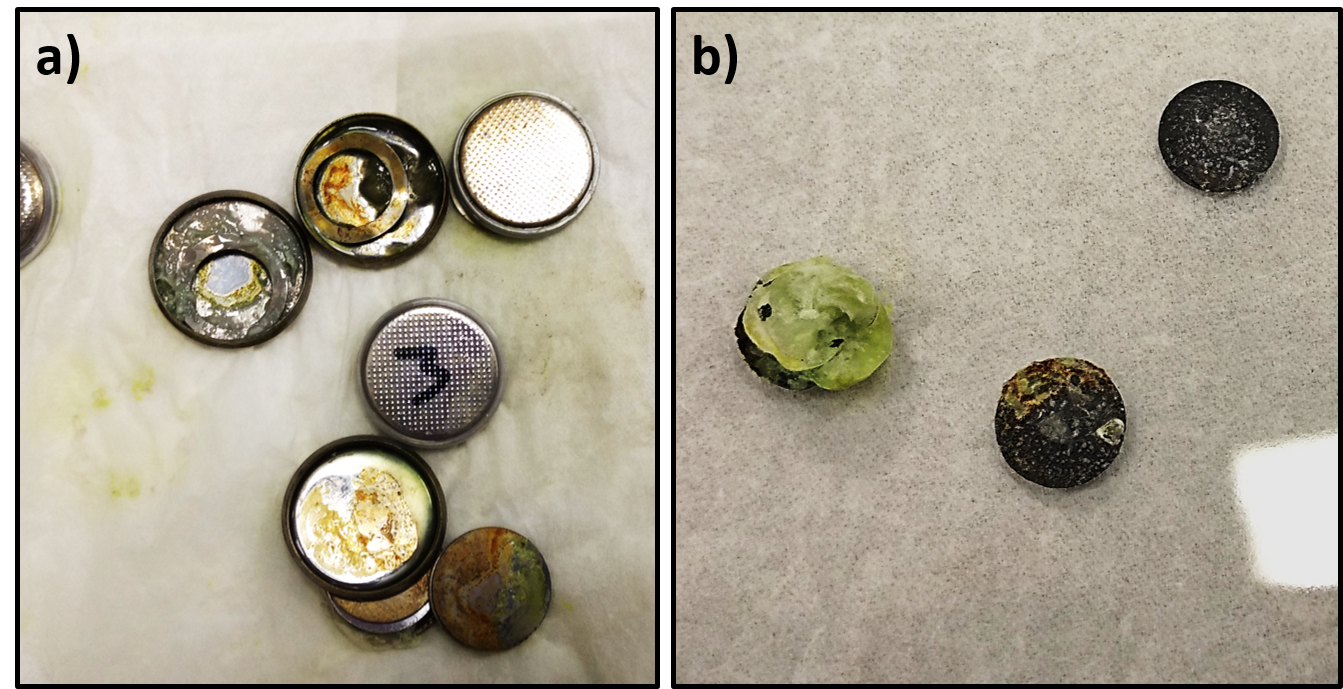
\includegraphics[width=\textwidth]{Figures/chap7fig/steeleffect}
\caption{SEM images of pristine hBN cathodes using a) DMSO, b) DMA, c) DMF and d) NMP solvents.}
\label{Figures/chap7fig:steeleffect}
\end{figure}
\begin{figure}[tbh!]
\centering
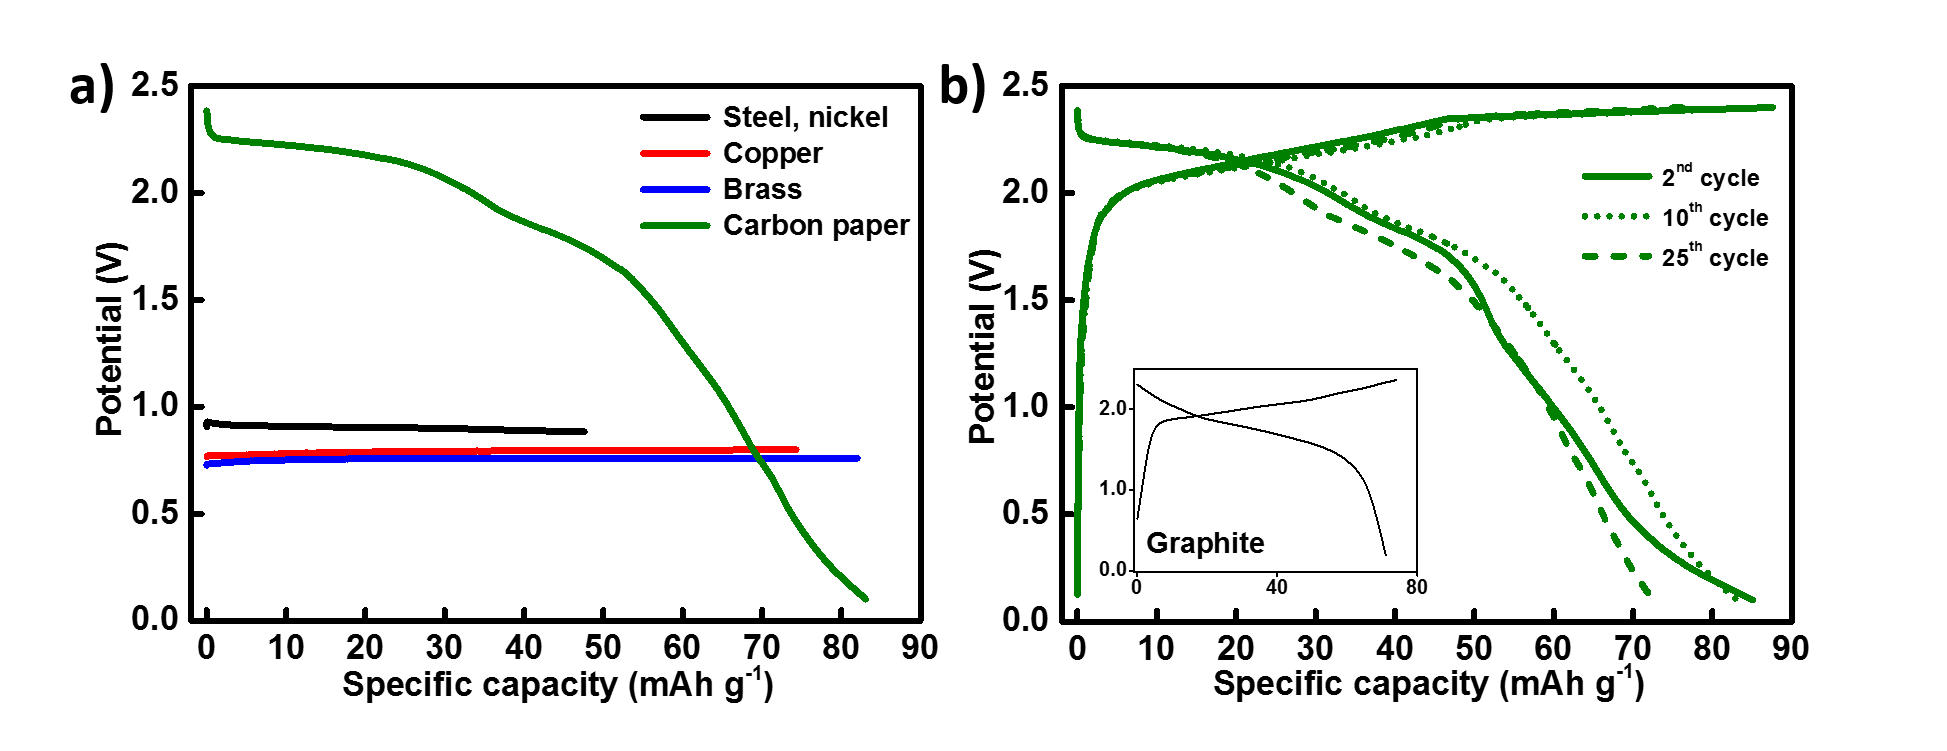
\includegraphics[width=\textwidth]{Figures/chap7fig/hBNCCCDC}
\caption{Galvanostatic cycles using hBN as the active material with a) steel and nickel foils (black), copper sheet (red), brass sheet (blue) and carbon paper (green) as current collectors in a two-electrode setup at a current rate of 40 mA g$^{-1}$. b) Performance of Al/hBN cell using carbon paper as the current collector which showed graphite dominating as active material (inset: CDC curve of an Al/graphite cell) }
\label{Figures/chap7fig:hBNCCCDC}
\end{figure}
\section{Conclusion and future outlook}
Replacing NMP with a cheaper solvent would be beneficial when commercialising AIBs. However, no solvent has proven to be as efficient as NMP yet. LIB plants recycle NMP on a regular basis. During vacuum drying process, NMP is collected from the exhaust gases and is used to clean equipment and is reused. This method can be applied while manufacturing AIBs, which would further reduce the battery production costs. 
Molybdenum, titanium and ITO turned out to be a good current collectors for our AIBs. Although a CC is inactive in a cell, however it occupies enough space- almost 9\%! If this number is reduced, the cell will record a higher energy density. One can use a thinner foil (structurally stable) instead of a thick one to attain a higher capacity value. In fact a thicker coating of the active material might seem as a solution but that limits the ion and electron transport across the electrode leading to a lower cycle life. 3D current collectors based on carbon might be the way to go. In LIBs, graphite foam has been used as a CC, since it does not intercalate at a potential >0.5V. Ruoff \textit{et al.}\cite{Ruoff} use graphene foam as a current collector for the first time. A 3D CC not only provides a dense interconnected structure that can rapidly transport /diffuse ions, but also an excellent conductivity. CC with a large pore volume accommodates expansion of active material would also prevent cathode pulverisation. 
